\chapter{Energy-Based Models}
% Authors: Bofeng Hu (Editor), Sakada Lim, Jialing Liao
% Lecture  points e: 3/25/2019

\section{Introduction}
% Authors: Bofeng Hu (Editor), Sakada Lim, Jialing Liao
% Lecture date: 3/25/2019

The Energy-Based Models (EBM) approach provides a general framework for many machine learning algorithms. They are designed to deal with situations where the machine learning system does not just compute an output as in a feed-forward process, but computes an output as the result of some optimization.

There are two forms of EBM, one for supervised learning (conditional) and one for unsupervised learning (unconditional). The conditional models take $x$ and $y$ as input, while the unconditional models take only $y$ as input. Their outputs are scalars, $F(x,y)$ or $F(y)$.


\begin{figure}[htb]
    \centering
    \begin{subfigure}[b]{0.25\textwidth}
        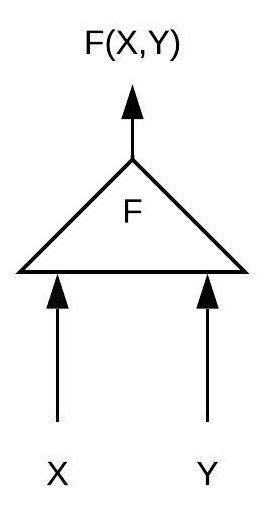
\includegraphics[width=\textwidth]{lectures/07-b/images/1-2.jpeg}
        \caption{Conditional}
        \label{fig:conditional}
    \end{subfigure}
    \begin{subfigure}[b]{0.27\textwidth}
        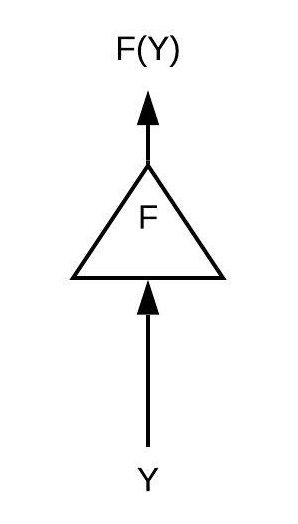
\includegraphics[width=\textwidth]{lectures/07-b/images/2-2.jpeg}
        \caption{Unconditional}
        \label{fig:unconditional}
    \end{subfigure}
    \caption{Two forms of Energy-Based Models}\label{fig:EBM}
\end{figure}

The output value indicates the ``compatibility'' of the input. In the conditional case, assume we have a properly trained EBM, and we show it an image of a table and the label for table, we get a small value as output, indicating these two are compatible. If we use an image of a table and the label for car, then the output energy should be higher. In the unconditional case, there is only one input, and the model tells us if it "looks good". For example, if this model is trained on natural images (ImageNet), and we show it an image like those in ImageNet, we get a low energy. But if we show it noise or something not natural, we get a high energy.


The model can be viewed as an energy function $F$. Suppose $x$ and $y$ are both scalars, and the data points are two-dimensional like in ~\ref{fig:conditionalexample1} and ~\ref{fig:unconditionalexample1}. In the conditional case, We want a function that takes low values on observed points and high values elsewhere. The problem is that for the value of $x$ at the bar, there are two possible $y$. If we build a model, for example a neural network, and compute $y$, we can only get one value for $y$. How do we represent the fact that we have two $y$? One trick is that we go through an implicit function. When we want to parameterized a circle, we use $x^2+y^2=r^2$. We can design an energy function that looks like $(x^2+y^2-r^2)^2$, which takes value 0 on the circle and larger values inside or outside the circle. This is one problem EBM attempts to solve. In the unconditional case, instead of $x$ and $y$, we have two $y$. Instead of predicting $y$ from $x$, we might have to predict $y_1$ from $y_2$ or $y_2$ from $y_1$ or just how they are compatible with each other. 

\begin{figure}[htb]
    \centering
    \begin{subfigure}[b]{0.3\textwidth}
        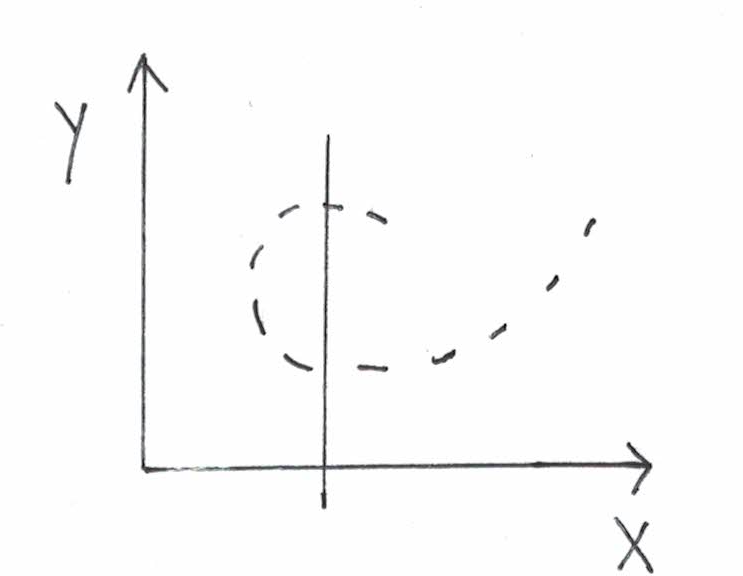
\includegraphics[width=\textwidth]{lectures/07-b/images/3.png}
        \caption{Conditional}
        \label{fig:conditionalexample1}
    \end{subfigure}
    \begin{subfigure}[b]{0.29\textwidth}
        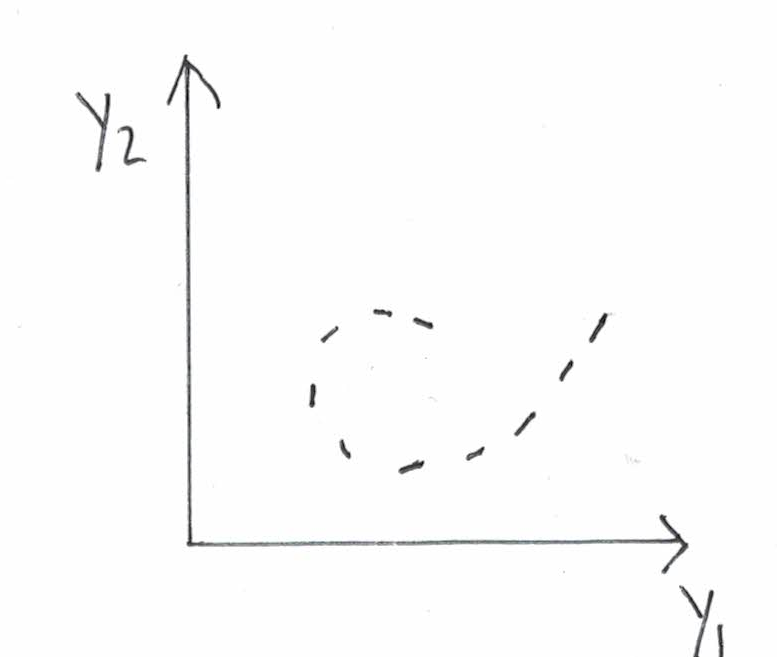
\includegraphics[width=\textwidth]{lectures/07-b/images/4.png}
        \caption{Unconditional}
        \label{fig:unconditionalexample1}
    \end{subfigure}
    \caption{Usage of EBM}\label{fig:Example1}
\end{figure}


For the above problems, we want some energy function that looks like \ref{fig:energyfunction}. The darker area represents the valley. When we move away from the valley, our energy goes up. For predicting $y$ from $x$, We can just find where our $y$ has the lowest energy.

\begin{figure}[htb]
  \centering
    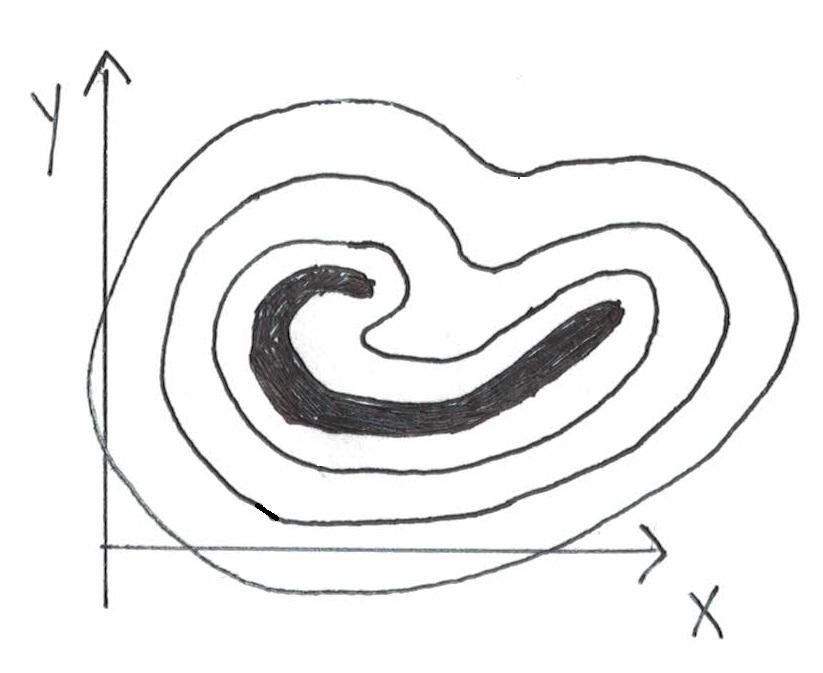
\includegraphics[width=0.3\textwidth]{lectures/07-b/images/5.png}
    \caption{Energy Function}
    \label{fig:energyfunction}
\end{figure}

\subsection{Relation with Probabilistic Models}
% Authors: Bofeng Hu (Editor), Sakada Lim, Jialing Liao
% Lecture date: 3/25/2019
If we want to turn an EBM into a probabilistic model, like $p(y|x)$. We can parameterized it with:


\begin{equation*}
    P(y|x) = \frac{e^{-\beta F(x,y)}}{\int_y e^{-\beta F(x,y)}}
\end{equation*}

Now we are turning an energy which we have not specified positive or negative into positive. Here the integral is over the entire space of $y$, so this is a normalized distribution over $y$. This is called the (Gibbs) Boltzmann distribution, which comes from statistical physics. This is a way of transforming an energy function into a distribution. But the normalization term is not always tractable. $y$ might be in high-dimension space. The energy function does not have a easy-to-compute integral, and so the normalization term is not computable. We have to use tricks like variational methods or Markov chain Monte Carlo. But this would make it complicated.

\subsection{Energy-Based Inference}
% Authors: Bofeng Hu (Editor), Sakada Lim, Jialing Liao
% Lecture date: 3/25/2019
In the conditional case, the inference process is to find a $y$ which minimizes this $F$ function. like

\begin{equation*}
    y^* = \argmin_y F_w (x,y)
\end{equation*}

Note that there can be multiple minima.

When designing the $F$ function, its range can be lower bounded, like the square function, so we know 0 is the floor, and can make it larger for other things. 

Another kind of inference would be returning a distribution over $y$ instead of a single $y$. But the machine has to be trained a particular way.

The $F$ function is not minimized during training, but instead during inference. For training, we shall minimize another loss function. We are going to parameterized F with w and train it.


\begin{figure}[htb]
    \centering
    \begin{subfigure}[b]{0.2\textwidth}
        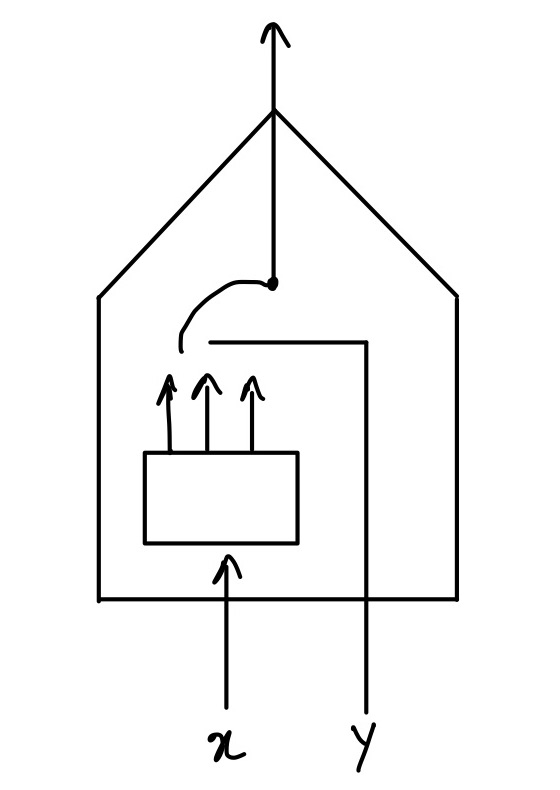
\includegraphics[width=\textwidth]{lectures/07-b/images/6-2.jpg}
        \caption{Conditional}
        \label{fig:energybasedmodel1}
    \end{subfigure}
    \begin{subfigure}[b]{0.2\textwidth}
        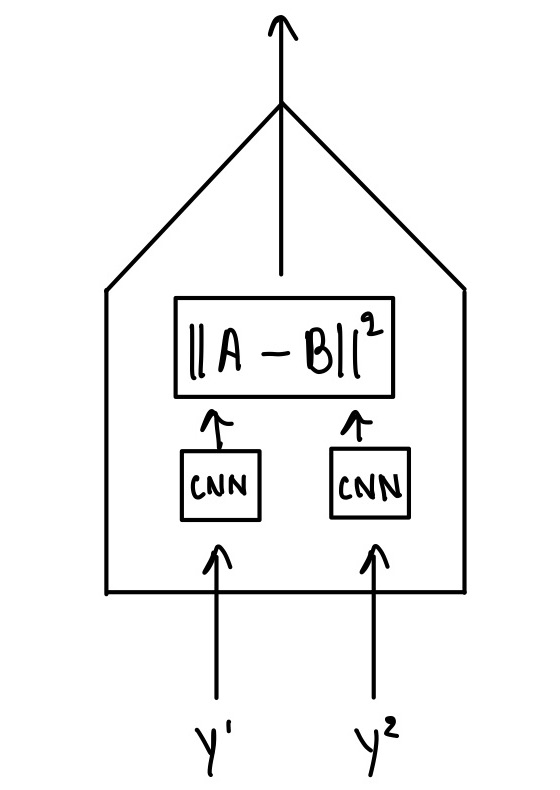
\includegraphics[width=\textwidth]{lectures/07-b/images/7-2.jpg}
        \caption{Unconditional}
        \label{fig:energybasedmodel2}
    \end{subfigure}
    \caption{Two examples of Energy-Based Models}\label{fig:Example2}
\end{figure}

In \ref{fig:energybasedmodel1}, the EBM takes an image, and run through a CNN which produces a bunch of scores for some categories. The $y$ is a discrete variable, which acts like a switch and chooses which output of the CNN is propagated to the final output. Suppose we have three categories: table, car, airplane. When we show it an image of car, and put car in $y$, it will select the output of car from the CNN, and return a score. A high score is bad, and a small score is good. If we put the label table, car and airplane in $y$, we select each of those, and get their scores. If we want to know which one it is, we find the one which gives the lowest energy, and this will be the answer.

In \ref{fig:energybasedmodel2}, we feed two vectors $y_1$ and $y_2$, and ask the system if they are compatible. We run them both through CNN, and compute the distance between the two outputs. This can be used in a face detector, where the model gives low energy for faces of the same person and high energy for faces of different person.

\section{Energy-Based Training}
% Authors: Bofeng Hu (Editor), Sakada Lim, Jialing Liao
% Lecture date: 3/25/2019
The training process should return a function like this: When we have training samples like $(x_i,y_i)$, we want $F(x_i,y_i)$ to be small. At the same time, we want $F(x_i,y_j)$ to be large, where $i \neq y$. For the unconditional case, we want $F(y_i)$ to be small.

\begin{equation*}
Conditional \begin{cases}
    F_w(x^i,y^i), & \text{small}.\\
    F_w(x^i,y^j), & \text{$i\neq j$,larger}.
    \end{cases}
\end{equation*}

\begin{equation*}
Unconditional \begin{cases}
    F_w(y^i), & \text{small}.\\
    F_w(y)& \text{$y\neq y^i$, larger}.\\
  \end{cases}
\end{equation*}

We need an objective function which push down the energy of training samples, and another term that pushes up the energy of everything else (outside the training samples). 

Suppose we want an energy function that looks like \ref{fig:energyfunction}. The training samples will be in the valley region. After getting a training sample, we can tweak the parameters of the energy function by gradient descent, so that the output energy goes down.

How do we push up the energy outside? We can generate samples outside and push them up. The space outside can be large, but this is what probabilistic approaches do.

Say we believe in maximum likelihood. Suppose we parameterized $p(y|x)$ with a Boltzmann distribution.

\begin{equation*}
    P_w(y|x) = \frac{e^{-\beta F_w(x,y)}}{\int_y e^{-\beta_w F(x,y)}}
\end{equation*}

We want to maximize the probability over the training samples

\begin{equation*}
    \prod_{i} P(y^i|x^i)
\end{equation*}

That is, we want to minimize the negative log of it.

\begin{equation*}
    L(w) = -\sum_i \log P(x^i | y^i)
\end{equation*}

That is our objective function. We plug in the distribution and rename this function, we get

\begin{equation*}
    \begin{split}
        L^{'}(w) & = \sum_i -\log \bigg\lbrack\frac{e^{-\beta F_w(x,y)}}{\int_y e^{-\beta_w F(x,y)}}\bigg\rbrack \\
        & = \sum_i [-\log e^{-\beta F(x,y)} + \log\int_y e^{-\beta F_w(x,y)}]
    \end{split}
\end{equation*}

\begin{equation*}
    \begin{split}
        L(w) & = \frac{1}{\beta}L^{'}(w) \\
        & = \sum_i [F_w (x^i,y^i) + \frac{1}{\beta}\log\int_y e^{-\beta F_w(x,y)}]
    \end{split}
\end{equation*}

When we try to minimize this, the first term tries to make the energy of the correct $y$ small, while the second term will make the energy of all $y$ high. 

If we compute the gradient with respect to $w$

\begin{equation*}
    \frac{\partial L(w)}{\partial w} = \sum_{i} [\frac{\partial F_{w}(x^i,y^i)}{\partial w} - \int_y P_{w}(y|x^i)\frac{\partial F_w(x^i,y)}{\partial w}]
\end{equation*}

where $P_w(y|X^i)$ is obtained through the Gibbs distribution.

There is a negative sign before the second term, which means it will increase the energy of all the y to some extent. More generally, what the gradient indicates is that, we are pushing down on the energy of the correct answer in the first term, and pushing up the energy of every answer, including the correct one, in the second term. And the force we push up a particular $y$ is proportional to the probability our model gives to that $y$. Note that the first term pushes down the energy of correct answers with a larger force.

If you have the energy function and can calculate the normalized term, then this is the way for maximizing the likelihood of the data, using the negative log-likelihood function.

If we take the EBM for \ref{fig:energybasedmodel1}, and we assume the probability of one $y$ given by the model is according to the Gibbs distribution. Suppose we try to push down the energy of the correct answers and push up the energy of the incorrect answers. Then this objective function becomes negative log-softmax, and this model is equivalent to a softmax on top of a neural network. We can also use other loss functions with similar results.

As it is difficult to parameterize $F$, we may use Monte Carlo methods to approximate the integral, for example using $\sum_{k} \frac{\partial F_w(x_i,y^k)}{\partial w}$. Another form of Monte Carlo is called Markov chain Monte Carlo (MCMC), where we have a sample $y$, and we modify the sample each time in such a way that every modification gives a sample that is more likely under the distribution. Another category for approximation is called variational methods, where we assume $P$ to have simpler form (e.g. Gaussian).

Basically, any object function that pushes down the energy of correct answers and pushes up the energy of incorrect answers will work. It may not be related to probabilities.